\chapter{Implementation of the Linux scheduler}
\label{chap:implementation}

\section{Structs and their role}

\paragraph{task\_struct}
As mentioned in chapter \ref{ch:introduction}, each task in the system is represented \newline by a  \verb|task_struct|, which contains all the information about it. Here we list some of the fields used by the scheduler, and then cover them in detail.
\begin{itemize}
    \item \verb|thread_info|. This struct is architecture dependant and can contain various fields. The most important for the scheduler is the \verb|flags| field. These flags are used to keep track of requests or signals from and for the task. \verb|TIF_SIGPENDING| means that the process has pending signals, \verb|TIF_MEMDIE| means that the process is being killed to reclaim memory. In particulare, there are two flags that are crucial for the scheduler: \verb|TIF_NEED_RESCHED| and \verb|TIF_POLLING_NRFLAG|. The first indicates that scheduling must be performed, and the second that the idle process is polling the \verb|TIF_NEED_RESCHED| flag.
    %from cesati's book
    \item \verb|state|. A long that represents the state of the task: -1 unrunnable, 0 runnable, $>0$ stopped. 
    \item \verb|on_rq|. Indicates if the process is on the runqueue.
    \item \verb|static_prio| and \verb|normal_prio|. The first is the priority used for real-time scheduling policies. If the task is scheduled under one of the normal scheduling policies \verb|static_prio| is set to zero and \verb|normal_prio| is used. This number is an internal representation used in the kernel, different from the priority value shown in user space.
    \item \verb|sched_entity|. This struct contains all the other information needed by the scheduler.
    \item Pointer to \verb|sched_class|. The scheduling class discussed in chapter \ref{ch:sched}. Contains a circular list of all scheduling classes.
    \item Pointer to \verb|mm_struct|. This struct represents the slice of virtual memory used by the process. Here, ``\verb|mm|'' stands for \textit{memory management}.
\end{itemize}

\paragraph{thread\_info}
This structure is very small and contains only basic information useful for scheduling, and each process has its own \verb|thread_info|. In figure \ref{img:stack} from chapter \ref{ch:introduction} it is shown that this struct is located at the bottom of kernel stacks. The small size of this struct is due to the fact that it has to fit in the small kernel stacks while not occupying too much space. Today, the implementation of \verb|thread_info| has changed: it is now embedded directly in \verb|task_struct|. 

\begin{code}
struct task_struct {
#ifdef CONFIG_THREAD_INFO_IN_TASK
	/*
	 * For reasons of header soup (see current_thread_info()), this
	 * must be the first element of task_struct.
	 */
	struct thread_info  thread_info;
#endif
// ...
\end{code}
With the previous implementation, \verb|thread_info| and \verb|task_struct| referenced each other through pointers. As shown in this code, if \verb|CONFIG_THREAD_INFO_IN_TASK| is defined, the field is not a pointer. With this new implementation, \verb|thread_info| is not located in the kernel stack. In order to access it, a pointer to the current task's \verb|thread_info| is saved, and its \verb|task_struct| can be accessed with the ``\verb|container_of()|'' trick discussed in chapter \ref{ch:introduction}. The implementation is very architecture dependent and this is specific to x86.

%TODO kernel preemption and user preemption, returning to user space (entry.S which defines entry and exit instruction)
%arch/x86/entry/entry_64.S explain kernel preemption e user preemption

%TODO explain TIF_NEED_RESCHED briefly (see cesati?)

\paragraph{sched\_entity}
The \verb|sched_entity| struct represent a \textit{schedulable entity}. From the scheduler's perspective, there is no difference between a process, a thread or even a whole group of processes: they are all just schedulable entities represented by this struct, and scheduler is oblivious to their real nature. Because of this, the scheduler works only with schedulable entities and not \verb|task_struct|s. For example, runqueues contain schedulable entities. 

A \verb|sched_entity| may be organized in a hierarchy of entities, this is done to allow group scheduling and it is optional. Suppose that there are more users using a system and we want to share the CPU equally between them, but they have different processes running. With normal CFS, each task is present in the runqueue and it is scheduled independently. By organizing the entities in hierarchies, we can group together the tasks and schedule them as a single schedulable entity. In the previous example we would have only two entities on the runqueue, one for each user, and a corresponding runqueue containing all the task of that user. The scheduler decides which of the two entities to schedule, as if there were only two tasks running, and then repeats the process for the sub-queue. As stated earlier, a \verb|sched_entity| does not always correspond to a process; only the leafs of this structure correspond to a task. 

The most important fields that compose \verb|sched_entity| are:
\begin{itemize}
    \item \verb|load_weight|. It contains the weight of the entity. The role of the weight is discussed in chapter \ref{ch:sched}.
    \item \verb|struct rb_node run_node|. Represents a node inside a red-black tree. The next section shows that the runqueue is organized as a red-black tree. This field is embedded in this struct because the implementation is similar to lists.
    \item \verb|on_rq|. Indicates if the entity is on the runqueue.
    \item \verb|exec_start|. The time at which the task started its execution on the CPU. %resetted each time (calc_delta_fair)
    \item \verb|sum_exec_runtime|. The total time that the task has actually spent running on the CPU before being weighted.
    \item \verb|vruntime|. The weighted total time that the task has spent running.
    \item \verb|struct sched_entity *parent|. The parent node in the hierarchy.
    \item \verb|struct cfs_rq *cfs_rq|. The runqueue on which this entity is queued.
    \item \verb|struct cfs_rq *my_q|. If this is a group, this is the sub-runqueue of this group. The children of this entity are queued here.
\end{itemize}
These fields are specific to CFS, where the runqueue is a red-black tree (\verb|rb_node| and \verb|cfs_rq|), and the timeslice is based on virtual runtime (\verb|exec_start| and \verb|sum_exec_runtime| are used to calculate vruntime). The other scheduling class have their own entity, such as \verb|sched_rt_entity| and \verb|sched_dl_entity|, defining its specific fields. \verb|sched_entity| is not called \verb|sched_fair_entity| supposedly because the fair class is the default. 

\paragraph{sched\_class}
This structure contains function pointers to the scheduler routines, specific to the scheduling class. Each class has routines that do the same thing, but with different implementations.

\begin{code}
struct sched_class {
	const struct sched_class *next; //Circular list of all classes

	void (*enqueue_task) (struct rq *rq, struct task_struct *p, int flags);
	void (*dequeue_task) (struct rq *rq, struct task_struct *p, int flags);
	void (*yield_task)   (struct rq *rq);
	bool (*yield_to_task)(struct rq *rq, struct task_struct *p, bool preempt);
	void (*check_preempt_curr)(struct rq *rq, struct task_struct *p, int flags);

	/*
	 * It is the responsibility of the pick_next_task() method that will
	 * return the next task to call put_prev_task() on the @prev task or
	 * something equivalent.
	 *
	 * May return RETRY_TASK when it finds a higher prio class has 
	 * runnable tasks.
	 */
	struct task_struct * (*pick_next_task)(struct rq *rq,
					       struct task_struct *prev,
					       struct rq_flags *rf);
    // ...
    void (*task_tick)(struct rq *rq, struct task_struct *p, int queued);
    void (*update_curr)(struct rq *rq);
    // ...
}
\end{code}
When scheduling, the class list is visited, starting from the higher priority class: if there is no process to schedule the next class is visited. This keeps going until something to schedule is found, then the correct function pointers are used to carry out the scheduler's jobs. 

This structure is a good reference to understand the code because it essentially lists all the main scheduler routines, which are covered in the next section.

\paragraph{mm\_struct} %TODO no code, see https://www.tldp.org/LDP/tlk/kernel/processes.html
%kernel threads have mm at null
%Need to explain mm_struct and some memory management (virtual memory and address spaces?)
\mycomment{TODO} mm switched during context switch

\begin{figure}[ht]
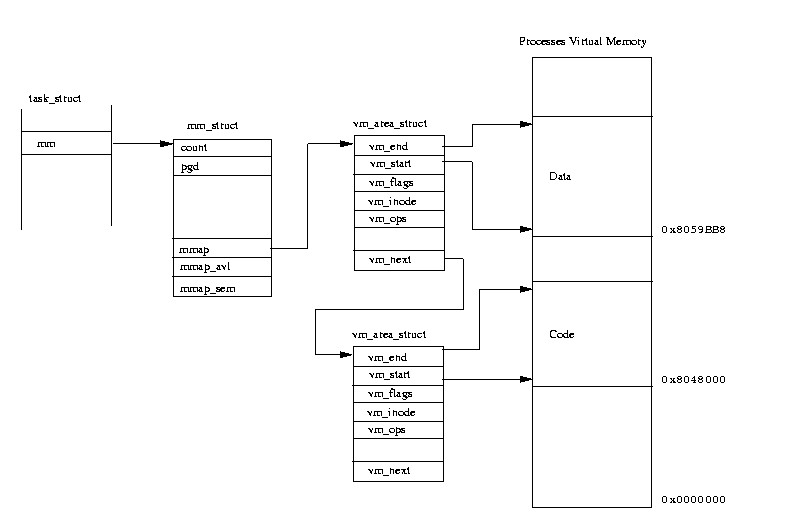
\includegraphics[width=\textwidth]{images/mm.jpg}
\caption{The structures used for virtual memory \url{https://www.tldp.org/LDP/tlk/kernel/processes.html}}
\label{img:mm}
\end{figure}

\paragraph{procfs}
The information contained in these structures can be accessed from outside the kernel with specific tools (covered in detail in Chapter \ref{chap:ftrace}). One approach to accomplish this it to use \verb|procfs|. In short, \verb|procfs| is a special filesystem that contains all the kernel information about processes, making it easy to access it from user space. For example, it is possible to gather scheduling information about process with pid 1196 by executing \verb|cat /proc/1196/schedstat|. This gives the following human-readable output:

\begin{verbatim}
tilda (1196, #threads: 3)
-------------------------------------------------------------------
se.exec_start                                :      26964101.112552
se.vruntime                                  :       2272975.687429
se.sum_exec_runtime                          :         10181.684621
se.nr_migrations                             :                11160
nr_switches                                  :                40529
nr_voluntary_switches                        :                40104
nr_involuntary_switches                      :                  425
se.load.weight                               :              1048576
se.avg.load_sum                              :              2453334
se.avg.util_sum                              :              2417183
se.avg.load_avg                              :                   45
se.avg.util_avg                              :                   45
se.avg.last_update_time                      :       26964101112552
policy                                       :                    0
prio                                         :                  120
clock-delta                                  :                   50
mm->numa_scan_seq                            :                    0
numa_pages_migrated                          :                    0
numa_preferred_nid                           :                   -1
total_numa_faults                            :                    0
current_node=0, numa_group_id=0
numa_faults node=0 task_private=0 task_shared=0 
group_private=0 group_shared=0
\end{verbatim}
Here, ``\verb|se|'' is the name of the field of type \verb|sched_entity| in \verb|task_struct|.

\paragraph{Red-black tree}
\label{sec:rb-tree}
The runnable tasks are stored inside a red-black tree, which allows more efficiency. A red-black tree is a type of self-balancing binary search tree: this means that the insertion and deletion operations will keep the height of the tree as small as possible. This characteristic is important because the cost of the most common functions (search, insertion and deletion) is proportional to the height of the tree.
As stated before, the task to run next is the one with the smallest vruntime. In a red-black tree, this corresponds to the task in the leftmost node. When picking the next task the tree is not traversed, instead, the leftmost node is cached in a dedicated variable in order to retrieve it faster.

\section{Time keeping}%correggi da qui
\label{sec:timekeeping}
Many functions of the kernel need to keep track of the passing of the time. The scheduler, for example, needs to know for how long a task has been running in order to know when to preempt it and give the control of the CPU to another task. But there are many other functions that are time-driven, so it's important to understand how the system keeps track of the time.

The kernel requires an hardware timer to manage the passing of time. This timer can be implemented in different ways and there can be more timers in a system, but the general idea is the same: the timer sends an interrupt at a fixed frequency known by the kernel, this way it also knows the time between two timer interrupts and can perform periodic actions such as updating the system uptime. The period between two interrupt is called a \textit{tick} and the frequency is called \textit{tick rate}, this value inside the kernel is defined as \textbf{HZ}. If the value of HZ is 100, it means that the frequency is 100HZ and there is a tick every $1/100$ seconds, or 10 milliseconds.

\subsubsection{Choice of the tick rate}
As we will see later, many parts of the system are time-dependant, so they rely on the timer interrupt. Changing the frequency of the interrupt can have a large impact on the behavior of the system, there are pros and cons to larger an smaller values oh HZ.

%pros of larger HZ
A larger HZ means that the timer interrupt has a finer resolution, which means that all the timed events also have a higher resolution and also allows to improve the accuracy of those events. As an example, let's consider process preemption, with an higher tick rate we can improve the accuracy and reduce the scheduling latency. Suppose that a process has 2 milliseconds left of its timeslice and the timer interrupt has just occurred, with an HZ of 100 the next interrupt will occur in 10 milliseconds, giving the process 8 extra milliseconds, it also means that another task has to wait for more time in the runqueue and this can be an issue for time-sensitive tasks. With a larger HZ, 1000 for example, in the worst case scenario, the latency is only 1 millisecond.

%cons of larger HZ
There is also a drawback to increasing the tick rate: the interrupt handler gets executed more often and results in less processor time for the tasks. The actual impact of the increased overhead is debatable and depends on the speed of the processor.

%different values of HZ
The value of HZ depends on the hardware and on the configuration of the machine. On i386 HZ had a value of 100, with linux version 2.6 the value was raised to 1000 and later was made a configurable parameter and the default became 250. With the time were also introduced other, more accurate, timers, making an high HZ less necessary. It is also possible to configure the kernel as \textit{tickless} (NO\_HZ), this means that the interrupt is no longer at fixed intervals, but it's dynamically scheduled as needed, which is helpful for power savings.

\subsubsection{Jiffies}
%What is jiffies
\textit{Jiffies} is the number of ticks that have occurred since the system started, very time that the interrupt handler is executed, the value of \textit{jiffies} is increased by one. This means that if we know the value of HZ and the value of jiffies we can theoretically convert from seconds to jiffies, simply by doing \verb|seconds * HZ| and from jiffies to seconds with: jiffies / HZ
%TODO: code for conversion here
%add more about implementation

\paragraph{sched\_clock()}
\label{sched_clock}
An important function of the kernel is \verb|sched_clock()|, it returns the system's uptime in nanoseconds. An architecture may provide an implementation, but if it is not provided, the system will use the jiffies counter to calculate the system's uptime.

The scheduler uses this function to determine the absolute time that the current task has been running. If the system uses the jiffies counter to determine this value the maximum resolution of \verb|sched_clock()| depends on the value of HZ. In this case the choice of HZ becomes more relevant.
The default implementation of \verb|sched_clock()| using jiffies is this:
\begin{code}
unsigned long long __weak sched_clock(void)
{
	return (unsigned long long)(jiffies - INITIAL_JIFFIES)
					* (NSEC_PER_SEC / HZ);
}
\end{code}

\subsubsection{Interrupt Handler}

As we said before, the interrupt handler gets called at fixed intervals (unless configured with NO\_HZ). The handler perform many important functions, some of this actions depend on the architecture of the system, but some are independent and are executed by the \verb|periodic_tick()| function (in \verb|kernel/time/tick_common.c|):

\begin{code}
static void tick_periodic(int cpu)
{
	if (tick_do_timer_cpu == cpu) {
		write_seqlock(&jiffies_lock);

		/* Keep track of the next tick event */
		tick_next_period = ktime_add(tick_next_period, tick_period);

		do_timer(1);
		write_sequnlock(&jiffies_lock);
		update_wall_time();
	}

	update_process_times(user_mode(get_irq_regs()));
	profile_tick(CPU_PROFILING);
}
\end{code}
The two most important functions here are \verb|do_timer(1)| and \verb|update_process_times|. The first one increments the value of jiffies and updates the load statistics for the system.

The second is the most important for the scheduler, it updates various statistics and updates the runtime of the current task, if the task has finished its timeslice, it prompts a reschedule. We will see later in more detail how this works.

\subsubsection{update\_process\_times()}
This function updates the time that the current process has been running, the process changes if the process was running in user mode or in kernel mode. Remember that \verb|task_struct| has two different fields \verb|utime| and \verb|stime| to keep track of time spent in user space and in kernel space respectively.

The other important thing this function does is invoking the \verb|scheduler_tick| function.

\section{Scheduler routines}

We will now analyze in more detail how the scheduling works and the most important functions involved. In the last section we saw how the system can perform periodic functions at fixed intervals to measure the passing time.

%If there are events in the fuction, explain them in the FTRACE section
%show trace starting from the timer interrupt, using function_graph tracer
Path that \verb|schedule()| takes. TODO
\begin{codebash}
#!/bin/bash
echo function_graph > /sys/kernel/debug/tracing/current_tracer
# removing noise to see just the actual function trace
#trace on cpu0 only (actually disables tracing on other cpus)
echo 1 > /sys/kernel/debug/tracing/tracing_cpumask 
#show comments on all exit points
echo funcgraph-tail > /sys/kernel/debug/tracing/trace_options 
# function to trace
echo $* > /sys/kernel/debug/tracing/set_graph_function
# clear previous trace
echo > /sys/kernel/debug/tracing/trace
sleep 3
cat /sys/kernel/debug/tracing/trace
\end{codebash}

\begin{Verbatim}
selected schedule() calls from the script here
\end{Verbatim}

\subsection{scheduler\_tick()}
As we mentioned in the previous section the \verb|scheuler_tick()|  function is called by the interrupt handler at every tick, this means that it is called with a frequency of HZ.

\begin{code}
void scheduler_tick(void)
{
	int cpu = smp_processor_id();
	struct rq *rq = cpu_rq(cpu);
	struct task_struct *curr = rq->curr;
	struct rq_flags rf;

	sched_clock_tick();

	rq_lock(rq, &rf);

	update_rq_clock(rq);
	curr->sched_class->task_tick(rq, curr, 0);
	cpu_load_update_active(rq);
	calc_global_load_tick(rq);
	psi_task_tick(rq);

	rq_unlock(rq, &rf);

	perf_event_task_tick();

#ifdef CONFIG_SMP
	rq->idle_balance = idle_cpu(cpu);
	trigger_load_balance(rq);
#endif
}
\end{code}

The first important function here is \verb|sched_clock_tick()|, this function updates the per-CPU \verb|sched_clock_data| struct. To update this time, it uses the \verb|sched_clock()| function discussed in the section before \ref{sched_clock}.

The \verb|sched_rq_clock()| updates the \verb|clock_task| field inside the \verb|task_stuct|, this is used later by \verb|update_curr()|.

It then invokes the \verb|task_tick| function for the current task that is running to update the statistics of the task. This action depends on the scheduling class that the current process is using. We will now see how the \verb|fair_sched_class| works.

\subsubsection{task\_tick\_fair}

The runtime statistics for the current process are stored in the \verb|sched_entity| associated with it. The scheduler updates its parameters and then check if the current task is to be rescheduled. 

Remember that entities can organized in hierarchies.
We can now analyze the \verb|task_tick_fair| function:
\begin{code}
static void task_tick_fair(struct rq *rq, struct task_struct *curr, int queued)
{
	struct cfs_rq *cfs_rq;
	struct sched_entity *se = &curr->se;

	for_each_sched_entity(se) {
		cfs_rq = cfs_rq_of(se);
		entity_tick(cfs_rq, se, queued);
	}

	if (static_branch_unlikely(&sched_numa_balancing))
		task_tick_numa(rq, curr);

	update_misfit_status(curr, rq);
}
\end{code}

This function fetches the \verb|sched_entity| of the current process running, this is going to be a leaf of the hierarchy, and, if the task isn't part of a group, it is also the root. Remember that the \verb|sched_entity| struct point to two runqueues: \verb|cfs_rq| and \verb|my_q|, the first is the runqueue on which the entity is scheduled, the second is the runqueue that belongs to that group. When the entity is a leaf the second field is empty. 

For each entity in the hierarchy starting from the leaf, it calls:
\begin{itemize}
    \item \verb|cfs_rq_of(se)|, which returns the runqueue on which the entity is scheduled, if the system is configured without group scheduling there is only one runqueue.
    
    \item then \verb|entity_tick(cfs_rq, se, queued)|, which updates the statistics of that entity and checks if it has finished its time and if another entity deserves to run. This means that if a process inside a group still deserves more time, but the entire group has finished its time and another group deserves the CPU, the task is preempted anyway. \verb|entity_tick| also updates the load statistics used to balance the load between CPUs.
\end{itemize}

\subsubsection{update\_curr()}

The first part of \verb|entity_tick()|'s job, updating the runtime statistics, it's done by the function \verb|update_curr()|. This function takes as argument only the runqueue on which the current task is running, returned by: \verb|cfs_rq_of(se)|. From the runqueue it gets the \verb|sched_entity| of the current task running. It also gets the current time from the runqueue's clock.

\begin{code}
static void update_curr(struct cfs_rq *cfs_rq)
{
	struct sched_entity *curr = cfs_rq->curr;
	u64 now = rq_clock_task(rq_of(cfs_rq));
	u64 delta_exec;

	if (unlikely(!curr))
		return;

	delta_exec = now - curr->exec_start;
	if (unlikely((s64)delta_exec <= 0))
		return;

	curr->exec_start = now;

	schedstat_set(curr->statistics.exec_max,
		      max(delta_exec, curr->statistics.exec_max));

	curr->sum_exec_runtime += delta_exec;
	schedstat_add(cfs_rq->exec_clock, delta_exec);

	curr->vruntime += calc_delta_fair(delta_exec, curr);
	update_min_vruntime(cfs_rq);

	if (entity_is_task(curr)) {
		struct task_struct *curtask = task_of(curr);

		trace_sched_stat_runtime(curtask, delta_exec, curr->vruntime);
		cgroup_account_cputime(curtask, delta_exec);
		account_group_exec_runtime(curtask, delta_exec);
	}

	account_cfs_rq_runtime(cfs_rq, delta_exec);
}
\end{code}

\verb|curr->exec_start| is the time at which the entity was selected by the scheduler to be executed. %pick_next_entity()->set_next_entity()->update_stats_curr_start()
We can calculate \verb|delta_exec|, the amount of time that the task has spent running, simply by subtracting \verb|exec_start| from the current time, this value is then used to update the total runtime of the entity (can correspond to a group or a task) and the longest execution.

The virtual runtime is calculated by \newline \verb|__calc_delta(delta, NICE_0_LOAD, &se->load);|. %explain

If the newly calculated vruntime is also the smallest in the runqueue, the field \verb|cfs_rq->min_vruntime()| is updated.

\verb|update_curr()| also triggers the event \verb|sched_stat_runtime|\label{trace:sched_stat_runtime}, this event signals when a process's virtual runtime is updated.

It is also possible that a group of tasks has a limit on the amount of CPU it can use. The function \verb|account_cfs_rq_runtime| updates \newline \verb|cfs_rq->remaining_runtime|, where \verb|cfs_rq| is, again, the runqueue of the current group, and also triggers a reschedule if the remaining time reaches zero.

\subsubsection{check\_preempt\_tick()}

The job of \verb|check_preempt_tick()| is to check if the current task has to be preempted. The first step is calculating \verb|ideal_runtime|, as the name suggests, this is the time that is assigned to the task. It's calculated by \newline \verb|__calc_delta(slice, se->load.weight, load)| where the first argument is the target latency, the second is the weight of the entity and the third is the total load of the current runqueue. This function calculates the \verb|assigned_time| of formula \ref{eq:2.4}.

If the task has run for more than the ideal runtime, the function \verb|resched_curr()| is called and it will cause the preemption of the task.

The other way it can trigger a reschedule is if the difference between the virtual runtime of the current task and the smallest virtual runtime in the runqueue is bigger than the ideal runtime.
%what is the difference between the 2 cases? just the buddies?

\paragraph{resched\_curr()}\label{resched_curr}
This function simply sets the \verb|TIF_NEED_RESCHED| which indicates that the current task needs to be rescheduled. When resuming the execution of a user process, the flag is check and if it is set, the schedule function is called, this will select the next task to run.
%explain wake_idle_without_ipi and when it is called

\subsection{Adding a task to the runqueue}

A task can be added to the runqueue in 2 cases: when it is created, when it is woken up after sleeping.

Let's start by describing what happens when a new task is created via the \verb|fork()| system call.

\subsubsection{A new process is created}
When a process calls \verb|fork()| its \verb|task_struct| is duplicated and a new process is started. This is done by the \verb|_do_fork()| function that also triggers the \verb|sched_process_fork|\label{trace:sched_process_fork} event. It then calls the function \verb|wake_up_new_task()| that takes as argument the newly created \verb|task_struct|.

This function sets the state of the task as \verb|TASK_RUNNING|, then, after initiating some values used for scheduling statistics, invokes the \verb|activate_task()| function that will proceed in activating the task. After the task has been activated and placed on the runqueue, \verb|wake_up_new_task| triggers the \verb|sched_wakeup_new| \label{trace:sched_wakeup_new} event. Lastly this function calls \verb|check_preempt_curr()| that has the job of preempting the current task if another is more deserving. 

\paragraph{check\_preempt\_curr()}\label{check_preempt_curr}
This function compares the newly created task with the one currently running. The first thing it has to check is the scheduling class. A task of a lower priority scheduling class cannot preempt one of an higher class. On the other hand if the new task has an higher priority, the \verb|resched_curr()| function is called that will cause the task to be rescheduled.

When the two tasks have the same scheduling class, the decision depends on the class. If they use the \verb|fair_sched_class| the \newline \verb|check_preempt_wakeup()| function in \verb|fair.c| is called.

If the current task's policy is \verb|SCHED_IDLE| and the new task has a different policy, then the old task is preempted. Also, a batch or an idle task cannot preempt a non-idle task. If the tasks have the same policy, the virtual runtime of the current task is updated and then compared with the virtual runtime of the new task.

\begin{code}
static int
wakeup_preempt_entity(struct sched_entity *curr, struct sched_entity *se)
{
	s64 gran, vdiff = curr->vruntime - se->vruntime;

	if (vdiff <= 0)
		return -1;

	gran = wakeup_gran(se);
	if (vdiff > gran)
		return 1;

	return 0;
}
\end{code}

If the current task has a smaller virtual runtime than the new one, the task is not preempted. Otherwise it is preempted if the difference between the virtual runtimes is big enough. This is done to avoid too frequent rescheduling. 

The scheduler has a tunable parameter called \verb|wakeup_granularity| that controls the minimum difference necessary to preempt the task. This value is not directly used, instead it's first weighted by the weight of the new task with the \verb|calc_delta_fair()| function.  This is the same function used to calculate the virtual runtime. The new task is used, instead of the current one, because this penalizes tasks with smaller weights:
\begin{itemize}
    \item if the new task has a smaller weight than the current one, then the corresponding weighted granularity will be larger. This means that it is harder for the new task to preempt the current one.
    
    \item on the contrary, if the new task has a larger weight, it will be easier to preempt the current task. 
\end{itemize}

If the current task needs to be rescheduled, the \verb|check_preempt_wakeup()| function, calls \verb|set_next_buddy()| that tells to scheduler to favor the newly added task when choosing the next task. Finally the \verb|resched_curr()|\ref{resched_curr} function is called.

\subsubsection{A task is woken up}

Waking up a process is similar to creating a new one: the task is first inserted into the runqueue and then the system checks if the currently running task needs to be rescheduled.

Before inserting the task into the runqueue, the \verb|sched_waking|\label{trace:sched_waking} event is triggered and the task's state is set to \verb|TASK_WAKING|. The task is then inserted into the runqueue by \verb|activate_task()|. Once it is on the runqueue the \verb|task_struct->on_rq| field  is set to \verb|TASK_ON_RQ_QUEUED|. Finally the function \verb|ttwu_do_wakeup()| is called, which checks if the current task can be preempted with \verb|check_preempt_curr()|\ref{check_preempt_curr}, sets the task's state to \verb|TASK_RUNNING| and triggers the \verb|sched_wakeup|\label{trace:sched_wakeup} event.

\subsubsection{enqueue\_task()}
Whether the task was just created or it was woken up from sleep, his \verb|task_struct| has to be added to the runqueue. This is done by the \verb|enqueue_task()| function. It takes as arguments a pointer \verb|rq| to the runqueue in which to insert the task, a pointer \verb|p| to the \verb|task_struct| and an int representing the flags. It updates the \verb|cfs_rq| utilization statistics and invokes the \verb|enqueue_entity()| function that:
\begin{itemize}
    \item calls \verb|updats_curr()| adds \verb|cfs_rq->min_vruntime| to \verb|se->vruntime|, otherwise the new task would have too large boost compared to running tasks. Note that the virtual runtime is decreased when dequeuing a task.
    \item updates the load statistics of the entity and its group
    \item if \verb|ENQUEUE_WAKEUP| calls \verb|check_spread|
    \item calls \verb|__enqueue_entity()| that insert the entity in the red-black tree representing the runqueue.
\end{itemize}

% TODO
% \subsubsection{schedule()}

% \subsubsection{context\_switch()}

% in cfs_rq
%     struct sched_entity	*curr;
% 	struct sched_entity	*next;
% 	struct sched_entity	*last;
% 	struct sched_entity	*skip;
